\documentclass{standalone}
\usepackage{pgf}
\usepackage{amsmath}
\usepackage{tikz}
\usetikzlibrary{shapes,arrows}
\usetikzlibrary{positioning}
\begin{document}
   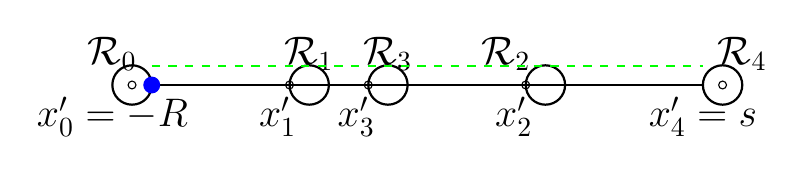
\begin{tikzpicture}

\coordinate(p0) at (-2.25,0);
\coordinate(p4) at (5.25,0);

\coordinate  (a) at (0,0);
\coordinate  (b) at (1,0);
\coordinate  (c) at (3.,0);


\draw[thick] (a) circle (0.25cm);
 \node[draw=none,align=left] at (0,0.4) {\Large $\mathcal{R}_1$};
\node[draw=none,align=left] at (-0.4,-0.4) {\Large $x_1'$} ;
\draw[black] (-0.25,0) circle (.05cm); 

\draw[thick] (b) circle (0.25cm);
 \node[draw=none,align=left] at (1,0.4) {\Large $\mathcal{R}_3$};
\node[draw=none,align=left] at (0.6,-0.4) {\Large $x_3'$} ;
\draw[black] (0.75,0) circle (.05cm); 


\draw[thick] (c) circle (0.25cm);
\node[draw=none,align=left] at (2.5,0.4) {\Large $\mathcal{R}_2$};
\node[draw=none,align=left] at (2.6,-0.4) {\Large $x_2'$} ;
\draw[black] (2.75,0) circle (.05cm); 

\draw[thick] (p0) circle (0.25cm);
 \node[draw=none,align=left] at (-2.5,0.4) {\Large $\mathcal{R}_0$};
\node[draw=none,align=left] at (-2.5,-0.4) {\Large $x_0'=-R$} ;
\draw[black] (-2.25,0) circle (.05cm); 

\draw[thick] (p4) circle (0.25cm);
 \node[draw=none,align=left] at (5.5,0.4) {\Large $\mathcal{R}_4$};
\node[draw=none,align=left] at (5.0,-0.4) {\Large $x_4'=s$} ;
\draw[black] (5.25,0) circle (.05cm); 



\draw[thick] (-2,0) -- (+5,0);


\draw[blue,fill=blue] (-2,0) circle (.1cm); 


\draw[dashed,thick,green] (-2,0.24) -- (5,0.24);


\end{tikzpicture}
\end{document}

